\chapter{Consuming Linked Data}
\label{ch:ch5}

\begin{itemize}
\item Contrib 1: Wizard for visualizations

\item Contrib 2: Vocabularies for describing visualizations

\item Contrib 4: Revealing the “important” properties of Entities for visualizations

\item Contrib 5: Focus on Event--Confomaton
\item Contrib 6: Focus on statistics -Concrete applications: PerfectSchool, French Amenities.

\item Contrib 7: Apps4Europe: Improving the discovery of application contests in Open Data Events


\end{itemize}


\section{A vocabulary for Describing VIsualization Applications} \label{sec:dvia}

We have implemented a vocabulary, DVIA\footnote{\url{http://bit.ly/Vb4L8k}} aims at describing any applications developed to consume datasets in 4-5 stars, using visual tools to showcase the benefits of Linked Data. It reuses four existing vocabularies: \texttt{Dublin Core terms} \footnote{\url{http://purl.org/dc/terms/}}, \texttt{dataset catalogue (DCAT)}\footnote{\url{http://www.w3.org/ns/dcat#}}, \texttt{Dublin Core Metadata Initiative}\footnote{\url{http://purl.org/dc/dcmitype}} and \texttt{Organization vocabulary}\footnote{\url{http://www.w3.org/ns/org#}}.  It is composed of three main classes : 

\begin{itemize}
\item \textbf{Application}: This class represents the application or the mashup developed for demo-ing or consuming data in LD fashion. It is subclass of \textbf{dctype:Software}
\item \textbf{Platform}: The platform where to host or use the application, could be on the Web (Firefox, Chrome, IE, etc..) or mobile (android, iOS, mobile ) or even desktop
\item \textbf{VisualTool}: Represents the tool or library used to build the application. 
\end{itemize}

The diagram of the main classes and properties is depicted in Figure \ref{visuGraphModel}. The current version of the vocabulary in Turtle format can be found at \url{http://www.eurecom.fr/~atemezin/datalift/visumodel/visu-vocab.ttl} .  Listing \ref{snapshot} is a snapshot of the description of the application which won the Semantic Web Challenge\footnote{\url{http://challenge.semanticweb.org/2012/winners.html}} in 2012, the \textit{EventMedia Live} application, described using DVIA vocabulary. It depicts apart from some metadata about the application (dct:title, dct:name, dct:issued, dct:creator and dct:license), the different visualization libraries integrated for building Eventedia Live (e.g.: Google API, Backbone, etc), as well as the operating systems where it is designed for, the different views/facets available in the application (map, charts, graphs, force-directed layout, ect) and the heteregeneous datasets used to implement it. 
\lstset{basicstyle=\scriptsize, backgroundcolor=\color{white}, frame=single, caption= {Snapshot in Turtle of the description of Event Media Live Application}, label=snapshot, captionpos=b}
\begin{lstlisting}

visuapp:eventMedia01
       a dvia:Application ; 
       dct:title "EventMedia Live"@en;   
       dvia:description "An application for reconciling Live events with media" ; 
       dvia:url <http://eventmedia.eurecom.fr> ; 
       dct:issued "2012-11-10"^^xsd:date ; 
       dvia:businessValue "not commercial" ;   
       dvia:keyword "events, media"^^xsd:string ; 
       dct:license <http://www.opendatacommons.org/licenses/pddl/1.0/> ; 
      dvia:platform [ a dvia:Platform ; 
			dct:title: "Desktop" ;
			dvia:preferredNavigator "Google Chrome" ; 
			dvia:alternativeNavigator "FireFox" ;
			dvia:system "Mac OS, Windows, Linux"^^string ] ; 
		
     dvia:usesTool [ a dvia:visualTool; dct:title "Google visualization Tool" ; 
	dct:description "Google visualization API" ; 
	dvia:accessUrl <https://developers.google.com/chart/interactive/docs/reference> ; 
	dvia:downloadUrl <http://www.google.com/uds/modules/gviz/gviz-api.js/> ] ;
    dvia:usesTool visuapp:visualTool02 ;
    dvia:consumes [ a dcat:Dataset; dct:title "BBC dump"] ; 
    dvia:consumes [ a dcat:Dataset; dct:title "last.fm scrapped dataset"] ;
    dvia:consumes [ a dcat:Dataset; dct:title "upcoming scrapped dataset"] ;
    dvia:consumes [ a dcat:Dataset; dct:title "eventful scrapped dataset"] ;
    dvia:consumes [ a dcat:Dataset; dct:title "Flickr scrapped dataset"] ;
    dvia:consumes [ a dcat:Dataset; dct:title "Music Brainz "] ;
    dvia:consumes [ a dcat:Dataset; dct:title "Foursquare Json file"] ;
    dvia:consumes [ a dcat:Dataset; dct:title "DBpedia"] ;
    dct:creator [foaf:mbox "khrouf@eurecom.fr"; foaf:name "Houda Khrouf"];
    dct:creator [foaf:mbox "vuk@eurecom.fr"; foaf:name "Vuk Milicik"];
    dct:creator [foaf:mbox "raphael.troncy@eurecom.fr"; foaf:name "Raphael Troncy"];
    dvia:view "map, chart, graph, force-directed layout" ; 
       .
	   ...
	
\end{lstlisting}

The full version of this sample description is available at \url{http://www.eurecom.fr/~atemezin/datalift/visumodel/eventMedia-sample.ttl}. The actual version of the DVIA intends to be small enough to cover the concepts that are needed to reuse partial or full parts of applications. 

\begin{figure}[!htbp]
  \begin{center}
    %\leavevmode
      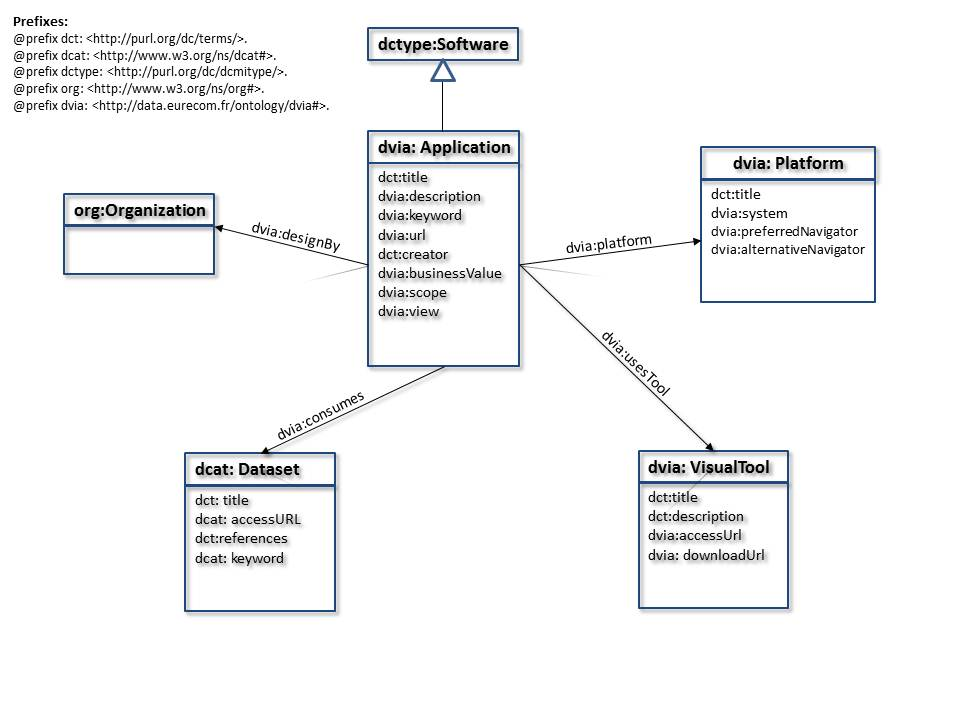
\includegraphics[ height=5in]{img/visuGraphModel.jpg}
  
    \caption{Conceptual Model of the DVIA vocabulary }
    \label{visuGraphModel}
  \end{center}
\end{figure}


\textcolor{red}{
\subsection{Conclusion} \label{sec:conclusion}
% deploy the vocab and setting up a hub for mashups
% find patterns for applications
% develop a recommender for creating applications according to some criteria
We have presented in this paper an approach that could help reusing tools and libraries in the domain of applications built on top of datasets in Linked Open Data. We first presented our motivation as to demonstrate to the end users or decision makers, there is always a need to develop a showcase, hence sometimes looking for analogous or similar applications in the area to ease the process of creation the mashup. We proceeded by surveying some applications to extract relevant common facts worth reusable, from which we proposed a small vocabulary (DVIA)  to semantically describe visual applications. 

We need to validate the DVIA by scrapping and reconciling data from all innovative applications websites and exposed them in RDF, starting with some of those we studied and others applications submitted at the Semantic Web Challenge the past three years. We strongly believe that having such a a hub  describing the tools, datasets, etc.  used to build  applications consuming 4-5 stars datasets will contribute to interoperable Applications leading to a Linked Open Visualizations (LOVIZ) on the LOD cloud.

Our ultime goal is to detect patterns used for creating Linked Data visual applications on the web using RDF data. For this challenge, we will need to perform some mining tasks of the underlying data (list of properties, number of triples, categories, etc.), the ontologies used, the templates or libraries for visualizations (Exhibit, GeoAPI, LDA, Sparkl, d3.js, etc) and finally evaluate the efforts for a user to build the application. This could lead to a framework for generating automatically visualizations from heterogeneous datasets by extracting relevant features combined to suitable templates tools for visualizations.}
